% This is "sig-alternate.tex" V2.0 May 2012
% This file should be compiled with V2.5 of "sig-alternate.cls" May 2012
%
% This example file demonstrates the use of the 'sig-alternate.cls'
% V2.5 LaTeX2e document class file. It is for those submitting
% articles to ACM Conference Proceedings WHO DO NOT WISH TO
% STRICTLY ADHERE TO THE SIGS (PUBS-BOARD-ENDORSED) STYLE.
% The 'sig-alternate.cls' file will produce a similar-looking,
% albeit, 'tighter' paper resulting in, invariably, fewer pages.
%
% ----------------------------------------------------------------------------------------------------------------
% This .tex file (and associated .cls V2.5) produces:
%       1) The Permission Statement
%       2) The Conference (location) Info information
%       3) The Copyright Line with ACM data
%       4) NO page numbers
%
% as against the acm_proc_article-sp.cls file which
% DOES NOT produce 1) thru' 3) above.
%
% Using 'sig-alternate.cls' you have control, however, from within
% the source .tex file, over both the CopyrightYear
% (defaulted to 200X) and the ACM Copyright Data
% (defaulted to X-XXXXX-XX-X/XX/XX).
% e.g.
% \CopyrightYear{2007} will cause 2007 to appear in the copyright line.
% \crdata{0-12345-67-8/90/12} will cause 0-12345-67-8/90/12 to appear in the copyright line.
%
% ---------------------------------------------------------------------------------------------------------------
% This .tex source is an example which *does* use
% the .bib file (from which the .bbl file % is produced).
% REMEMBER HOWEVER: After having produced the .bbl file,
% and prior to final submission, you *NEED* to 'insert'
% your .bbl file into your source .tex file so as to provide
% ONE 'self-contained' source file.
%
% ================= IF YOU HAVE QUESTIONS =======================
% Questions regarding the SIGS styles, SIGS policies and
% procedures, Conferences etc. should be sent to
% Adrienne Griscti (griscti@acm.org)
%
% Technical questions _only_ to
% Gerald Murray (murray@hq.acm.org)
% ===============================================================
%
% For tracking purposes - this is V2.0 - May 2012

\documentclass{sig-alternate-2013}


\usepackage{amsmath}
\usepackage{url}
\usepackage{graphicx}
\usepackage{subfigure}

\toappear{Submitted to SIGCSE 2016}

\newfont{\mycrnotice}{ptmr8t at 7pt}
\newfont{\myconfname}{ptmri8t at 7pt}
\let\crnotice\mycrnotice%
\let\confname\myconfname%

\permission{Permission to make digital or hard copies of all or part of this work for personal or classroom use is granted without fee provided that copies are not made or distributed for profit or commercial advantage and that copies bear this notice and the full citation on the first page. Copyrights for components of this work owned by others than ACM must be honored. Abstracting with credit is permitted. To copy otherwise, or republish, to post on servers or to redistribute to lists, requires prior specific permission and/or a fee. Request permissions from permissions@acm.org.}
\conferenceinfo{SIGCSE'15,}{March 4--7, 2015, Kansas City, MO, USA.\\
{\mycrnotice{Copyright is held by the owner/author(s). Publication rights licensed to ACM.}}}
\copyrightetc{ACM \the\acmcopyr}
\crdata{978-1-4503-2966-8/15/03\ ...\$15.00.\\
http://dx.doi.org/10.1145/2676723.2677284}

\clubpenalty=10000 
\widowpenalty = 10000


\begin{document}
%
% --- Author Metadata here ---
%\conferenceinfo{WOODSTOCK}{'97 El Paso, Texas USA}
%\CopyrightYear{2007} % Allows default copyright year (20XX) to be over-ridden - IF NEED BE.
%\crdata{0-12345-67-8/90/01}  % Allows default copyright data (0-89791-88-6/97/05) to be over-ridden - IF NEED BE.
% --- End of Author Metadata ---

%\toappear{To appear at SIGCSE 2015}

\title{Datathons: An Experience Report of Big Data Hackathons}

%
% You need the command \numberofauthors to handle the 'placement
% and alignment' of the authors beneath the title.
%
% For aesthetic reasons, we recommend 'three authors at a time'
% i.e. three 'name/affiliation blocks' be placed beneath the title.
%
% NOTE: You are NOT restricted in how many 'rows' of
% "name/affiliations" may appear. We just ask that you restrict
% the number of 'columns' to three.
%
% Because of the available 'opening page real-estate'
% we ask you to refrain from putting more than six authors
% (two rows with three columns) beneath the article title.
% More than six makes the first-page appear very cluttered indeed.
%
% Use the \alignauthor commands to handle the names
% and affiliations for an 'aesthetic maximum' of six authors.
% Add names, affiliations, addresses for
% the seventh etc. author(s) as the argument for the
% \additionalauthors command.
% These 'additional authors' will be output/set for you
% without further effort on your part as the last section in
% the body of your article BEFORE References or any Appendices.

\numberofauthors{2} %  in this sample file, there are a *total*
% of EIGHT authors. SIX appear on the 'first-page' (for formatting
% reasons) and the remaining two appear in the \additionalauthors section.
%
\author{
% You can go ahead and credit any number of authors here,
% e.g. one 'row of three' or two rows (consisting of one row of three
% and a second row of one, two or three).
%
% The command \alignauthor (no curly braces needed) should
% precede each author name, affiliation/snail-mail address and
% e-mail address. Additionally, tag each line of
% affiliation/address with \affaddr, and tag the
% e-mail address with \email.
%
% 1st. author
%\alignauthor
%Craig Anslow\\
%       \affaddr{Department of Computer Science}\\
%       \affaddr{University of Calgary}\\
%       \affaddr{Calgary, Alberta, Canada}\\
%       \email{craig.anslow@ucalgary.ca}   
%\alignauthor
%John Brosz\\
%       \affaddr{Taylor Digital Family Library}\\
%       \affaddr{University of Calgary}\\
%       \affaddr{Calgary, Alberta, Canada}\\
%       \email{john.brosz@ucalgary.ca}   
%\alignauthor
%Frank Maurer\\
%       \affaddr{Department of Computer Science}\\
%       \affaddr{University of Calgary}\\
%       \affaddr{Calgary, Alberta, Canada}\\
%       \email{frank.maurer@ucalgary.ca}   
%}
\alignauthor
Craig Anslow, John Brosz, Frank Maurer\\
       \affaddr{Department of Computer Science}\\
       \affaddr{University of Calgary}\\
       \affaddr{Calgary, Alberta, Canada}\\
       \email{\{canslow,jdlbrosz,fmaurer\}@ucalgary.ca}   
\alignauthor
Mike Boyes\\
       \affaddr{Department of Psychology}\\
       \affaddr{University of Calgary}\\
       \affaddr{Calgary, Alberta, Canada}\\
       \email{boyes@ucalgary.ca}   
}


\date{}
% Just remember to make sure that the TOTAL number of authors
% is the number that will appear on the first page PLUS the
% number that will appear in the \additionalauthors section.

\maketitle

\begin{abstract}
Hosting successful hackathons is difficult. With the accessibility of open data there is now an opportunity to host hackathons focused on big data, however these are new and not clearly defined about how to do this process. In this paper we present our experience at hosting three big data hackathons called \emph{datathons} that involved students and members from industry coming together to solve challenging problems with publicly open data and data from not for profits. The resources developed for our datathons about our experience will help inform others who also wish to host big data hackathons.
\end{abstract}

\category{K.3.2}{Computer and Information Science Education}{Computer science education}

\terms{Design}

\keywords{Big Data, Hackathon, Open Data}


%----------------------------------------------------
% INTRODUCTION
%----------------------------------------------------
\section{Introduction}

\section{Related Work}

% Hackathons 

Games and hackathons

% Experience of other hackathons

Stitch fest paper\cite{stitchfest}

% Big Data

explain what big data is

% we experimented with big data hackathons

explain we are exploring big data hackathons

\section{Datathons}


3. Datathons
- describe what a datathon is
3.1 Benefits
3.2 DFG Case Study
3.3 CODE Case Study
4. Discussion (Lessons Learned)
- community engagement
- participants: recruitment, group dynamics
- data: structuring and cleaning, open data, storing
- tools: analysis, visualization
- logistics: room setup, break out rooms, food
- things to avoid
5. Conclusions


 ? Intro
 ? Related Work
 ? Datathons in general
  ? benefits
  ? Two hackathon case studies
   � Code
    ? Recruitment - population of attendees
    ? Preparing data
    ? Setup
    ? Group dynamics
   � DfG
 ? Lessons Learned
  ? How to do, tips
  ? Things to avoid

%----------------------------------------------------
% PREPARATION and PLANNING
%----------------------------------------------------
\section{Preparation and Planning}

%----------------------------------------------------
% RECRUITMENT
%----------------------------------------------------
\subsection{Recruitment}

%----------------------------------------------------
% VENUE
%----------------------------------------------------
\subsection{Venue}

%\begin{figure}[!t] % this puts images exactly where you want them
%\begin{center}
%\subfigure[Expectations of the course from students.]{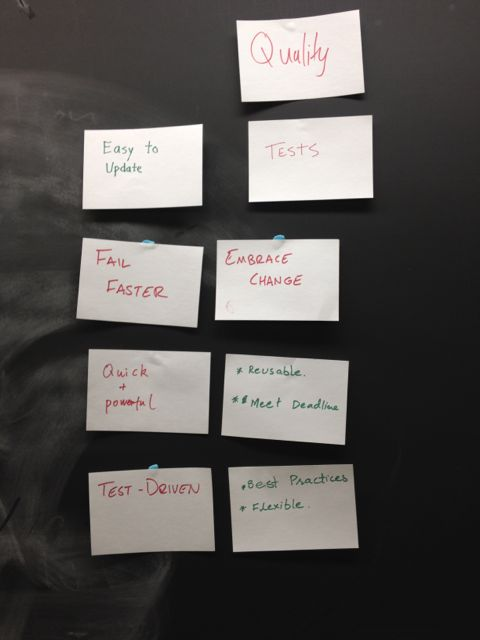
\includegraphics[keepaspectratio,width=4.1cm]{images/expectations.png}\label{fig:expectations}}
%\subfigure[Marshmallow Challenge: students working in teams.]{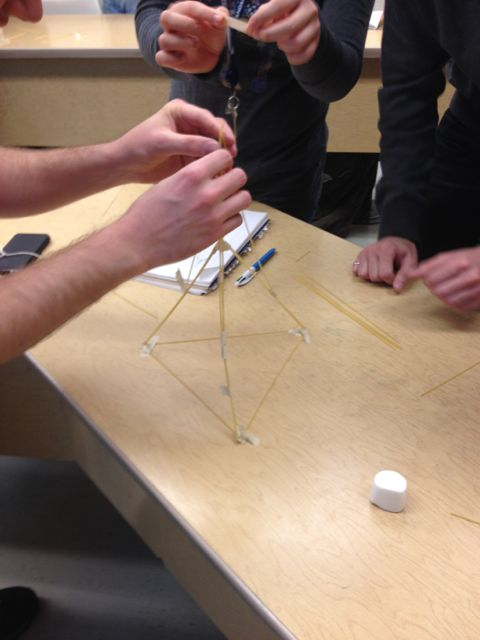
\includegraphics[keepaspectratio,width=4.1cm]{images/marshmallow.png}\label{fig:marshmallow}}
%\caption{Course Lectures - interactive exercises.}
%\label{fig:lectures}
%\end{center}
%\end{figure}
%

%----------------------------------------------------
% DATA PREPARATION
%----------------------------------------------------
\subsection{Data Preparation}

%----------------------------------------------------
% LOGISTICSs
%----------------------------------------------------
\subsection{Logistics}

%----------------------------------------------------
% HOSTING
%----------------------------------------------------
\section{Hosting the Event}

\section{Discussion}

\textbf{Participants.} recruitment, group dynamics, community engagement

\textbf{Data.} structuring and cleaning, open data, storing

\textbf{Tools.} analysis, visualization

\textbf{Logistics.} room setup, break out rooms, food

\textbf{Things to avoid.}
\section{Conclusions}


\section*{Acknowledgments}
\small
Thanks to the Government of Canada, City of Calgary for providing open data sets. Thanks to the Data For Good Calgary Meetup group for assisting with the datathon event.


\small
%
% The following two commands are all you need in the
% initial runs of your .tex file to
% produce the bibliography for the citations in your paper.

\bibliographystyle{abbrv}
\bibliography{abbrevs,myrefs}   % name your BibTeX data base
%\balancecolumns
\end{document}
